
\documentclass[10pt,letterpaper]{article}
% Default margins are too wide all the way around. I reset them here
%\setlength{\topmargin}{-.5in} \setlength{\textheight}{9in}
%\setlength{\oddsidemargin}{.125in} \setlength{\textwidth}{6in}

\usepackage{setspace}
\doublespacing

\usepackage{geometry}
\geometry{legalpaper, margin=1in}

\usepackage{pslatex}
\usepackage{apacite}
\usepackage{url}
\usepackage{array}
\usepackage{graphicx}
\usepackage{caption}
\usepackage{subcaption}
\usepackage{listings}
\usepackage{color}
\usepackage{textcomp}
\usepackage{amsmath}
\usepackage{amssymb}
\usepackage{wrapfig}
\usepackage{lipsum}


\newcolumntype{L}[1]{>{\raggedright\let\newline\\\arraybackslash\hspace{0pt}}m{#1}}
\newcolumntype{C}[1]{>{\centering\let\newline\\\arraybackslash\hspace{0pt}}m{#1}}
\newcolumntype{R}[1]{>{\raggedleft\let\newline\\\arraybackslash\hspace{0pt}}m{#1}}


\graphicspath{{figures/}}

\def\signed #1{{\leavevmode\unskip\nobreak\hfil\penalty50\hskip2em
  \hbox{}\nobreak\hfil(#1)%
  \parfillskip=0pt \finalhyphendemerits=0 \endgraf}}

\newsavebox\mybox
\newenvironment{aquote}[1]
  {\savebox\mybox{#1}\begin{quote}}
  {\signed{\usebox\mybox}\end{quote}}


 \newcommand{\denote}[1]{\mbox{ $[\![ #1 ]\!]$}}

\definecolor{Red}{RGB}{255,0,0}
\newcommand{\red}[1]{\textcolor{Red}{#1}}  

\usepackage{titlesec}

\setcounter{secnumdepth}{4}

\titleformat{\paragraph}
{\normalfont\normalsize\bfseries}{\theparagraph}{1em}{}
\titlespacing*{\paragraph}
{0pt}{3.25ex plus 1ex minus .2ex}{1.5ex plus .2ex}



\title{Generic supplement}


\begin{document}

\maketitle



\appendix


\section{Experiment 1a: \emph{Measuring $P(x)$ for familiar categories}}

The goal of this experiment was to measure participants' beliefs about the distributions of the prevalence of various properties.

\subsection{Participants}

We recruited 30 participants over Amazon's crowd-sourcing platform Mechanical Turk (MTurk).  Participants were restricted to those with US IP addresses and with at least a 95\% MTurk work approval rating. All participants were native English speakers. The experiment took about 10 minutes and participants were compensated \$1.00.

\subsection{Procedure and materials}

On each trial of the experiment, the participant filled out a table where each row was an animal category and each column was a property\footnote{The experiment in full can be viewed at \url{http://stanford.edu/~mtessler/experiments/generics/experiments/real-kinds/prior-2.html}}. 
Participants were asked to respond with the percentage of the species that had the property.
The list of animal categories was only partially pre-specified with animal categories that would be used in the generic truth judgment task.
%These names were randomly sampled from a larger set of categories of interest (see Appendix \ref{sec:appendix} for full list of animals and properties used). 
Participants were asked to add five of their own animal names to the list. 
Upon completion, the next column appeared with a property (e.g. ``has manes'') as the column header and text-boxes where the participants could put their estimated prevalence. 
%Participants were asked: ``For each kind of animal, what percentage of the species do you think [property]?'' 
This procedure was repeated for 8 properties in total. 
The animal kind column was unable to be modified once completed. 
The prevalence columns, however, could be modified at a later stage (i.e. the participant could go back and change her estimates after seeing more properties). 
Participants completed this procedure on each of 2 trials.

We used a set of properties associated with generics of theoretical interest (16 properties in total), motivated in part by conceptual distinctions pointed out by \citeA{Prasada2013}. 
The conceptual categories used to generate the generics were: majority characteristic (e.g. ``Leopards have spots''), minority characteristic (e.g. ``Lions have manes''), striking (e.g. ``Sharks attack swimmers.''), and majority false generalizations (e.g. ``Ducks are female.'') \cite{Prasada2013}. In addition, we included false sentences (e..g ``Lions lay eggs''), to cover the full range of possible truth values .
For a full list of the generic sentences used in this experiment, see Appendix \ref{sec:appendix}.
Complete instructions given to participants can be seen in Appendix \ref{sec:prior1instruct}.



\subsection{Bayesian data analysis}
\label{sec:bda1}

There is important latent structure in the prior elicitation task. We will describe the model from the perspective of inferring the distribution of a particular property (e.g. ``has manes''). 
The same general structure is implemented for each item independently. 

Responses $d$ can be categorized into those that reflect the property is either present or absent in the species. 
If the property is absent, then the response is 0\% (of the species has the property). 
The number of 0 responses act as an indicator of the prevalence of the property \emph{across categories} $\theta_{across}$ (for example, ``are male'' would have very few 0\% responses, whereas ``has manes'' would receive appreciably more, owing to the fact the prevalence of these properties \emph{across categories} is different).
%
\begin{align*}
d_{across} & \sim \text{Bernoulli}(\theta_{across}) \\
d_{across} & = \begin{cases}
				1 & \mbox{if } d > 0 \\
				0 & \mbox{if } d = 0 
				\end{cases}
\end{align*}
%
For those responses that reflect the property is present ($d > 0$), we assume those responses come from a distribution with unknown mean ($\gamma_{within}$) and variance ($\delta_{within}$). 
Since the responses vary between 0 - 100, the natural distribution is a Beta distribution. 
%We model the observed data as being generated by a mixture of this model and a model of random guessing behavior. 
%Modeling random guessing explicitly is important for recovering reliable estimates of the parameters of the model, which would otherwise be contaminated by this data \cite{LW2014}. 
%
\begin{align*}
d_{within} & \sim \text{Beta}(\gamma_{within}, \delta_{within})  \mbox{ if } d_{observed} > 0
\end{align*}
%
%\begin{align*}
%d_{within} \sim \begin{cases}
%					\text{Beta}(\gamma_{within}, \delta_{within})  &  \mbox{ if } d_{observed} > 0 \text{ and }  \text{Bernoulli} (\phi) = 0 \\
%					\text{Uniform}(0,1) & \mbox{ if } \text{Bernoulli} (\phi) = 1
%				\end{cases}
%\end{align*}
%
%In principle, $\phi$ could be vary by participant (some participants produce noisier data than others). For simplicity, we assume some global ``guessing rate'', and thus $\phi$ is an experiment-wide variable.
%We make no assumptions about the amount of noise in the data and 
We put uninformative priors over the means and concentrations of the prevalence distributions.  As well, we assume nothing \emph{a priori} about the prevalence across categories. 
%
\begin{align*}
% \phi \sim \text{Uniform}(0,1) \\
\theta_{across} \sim \text{Uniform} (0, 1) \\
\gamma_{within} \sim \text{Uniform}(0, 1) \\
\delta_{within} \sim \text{Uniform}(0, 50)
\end{align*}
%
We implemented this Bayesian statistical model using the probabilisitic programming language WebPPL \cite{dippl}. 
We used the Metropolis-Hastings algorithm to estimate the posterior distribution over the latent parameters $\theta_{across}, \gamma_{within}$, and $\delta_{within}$ with 3 chains of 100,000 iterations removing the first 50,000 iterations.

To reconstruct the likely distribution of  prevalence reflecting both within- and across- category prevalence, we took samples from the posterior predictive distribution of $d$ by running the forward model: 
%
\begin{align*}
h & \sim \text{Bernoulli}(\theta_{across}) \\
x & \sim \begin{cases} 
		\text{Beta}(\gamma_{within}, \delta_{within}) &\mbox{if } h = 1 \\ 
				0 & \mbox{if } h=0
				\end{cases} 
\end{align*}
%
where, $h$ is a variable indicating whether or not the property is present within a particular species. 

We also estimated the likely prevalence of each animal category and property pair of interest (e.g. the prevalence of ``has manes'' among ``Lions''), to be used as the measure of prevalence in the generic truth judgment task (Expt.~1b). 
For this, we assume the data was generated from a Beta distribution with unknown mean and concentration. 
%We also assume some global amount of noise in the data.

%\begin{align*}
%d \sim \begin{cases}
%					\text{Beta}(\gamma, \delta)  &  \mbox{ if } \text{Bernoulli} (\phi) = 0 \\
%					\text{Uniform}(0,1) & \mbox{ if } \text{Bernoulli} (\phi) = 1
%				\end{cases}
%\end{align*}
\begin{align*}
d \sim \text{Beta}(\gamma, \delta) 
\end{align*}



\section{Experiment 1b: \emph{Truth judgments of natural cases}}

The goal of this experiment was to measure participants' beliefs about the acceptability of a number of different generic sentences. 

\subsection{Participants}

We recruited 100 participants over Amazon's crowd-sourcing platform Mechanical Turk (MTurk).  Participants were restricted to those with US IP addresses and with at least a 95\% MTurk work approval rating. All participants were native English speakers. The experiment took about 3 minutes and participants were compensated \$0.35.

\subsection{Procedure and materials}

We used a two-alternative forced-choice (2AFC) paradigm to measure participants' beliefs about the acceptability of 30 generic sentences. 
Data reported in \citeA{Prasada2013} revealed that participants assign midpoint ratings on a Likert scale to anomalous generics like ``Birds are female''. 
We hypothesized that these ``neither true nor false'' ratings would be translated into more graded responses across the population using the 2AFC (i.e. subjects would be closer to chance).

Participants were asked to report whether they agreed or disagreed with generic sentences presented in bare plural form (e.g. ``Birds lay eggs.''). 
Items were presented sequentially, and participants reported whether or not they agreed with the sentence by pressing either ``P'' or ``Q'' (randomized between-subjects). 

Generic sentences were selected to correspond with the prevalence distributions elicited in Expt.~1a. 
They covered a range of conceptual categories: Characteristic (e.g. ``Ducks have wings.''), Minority (e.g. ``Lions have manes.''), Striking (e.g. ``Mosquitos carry malaria.''), False generalization (e.g. ``Lions are male.''), and false (e.g. ``Lions lay eggs.'').
Approximately 10 true, 10 false, and 10 uncertain truth-value generics were selected (see Appendix \ref{sec:appendix} for full list of items).
As a manipulation check, participants were asked at the end of the trials which button corresponded to ``Agree''.

\subsubsection{Results}

Four participants were excluded for failing to successfully report which button corresponded with ``Agree''. 
Five additional participants were excluded for listing a language other than English as their native language, resulting in 91 participants.

%\begin{figure}
%\centering
%    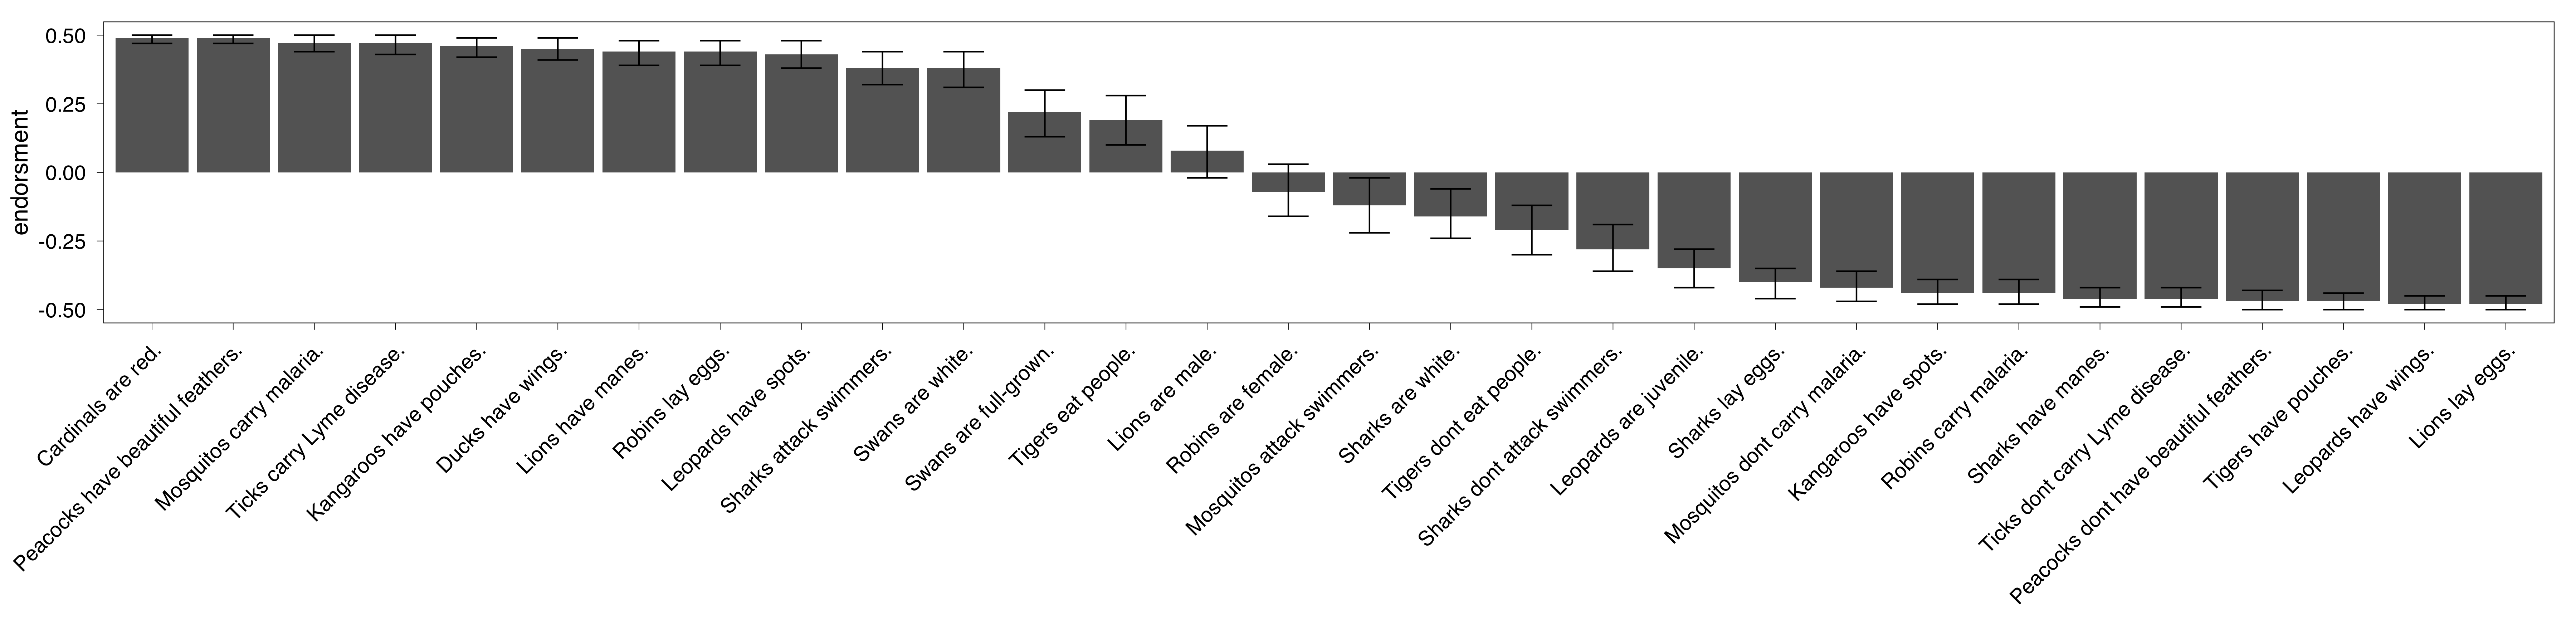
\includegraphics[width=\columnwidth]{truhtjudge_n100}
%    \caption{Truth judgments from Expt.~1b for each item. Y-axis denotes deviations from chance in the 2AFC. There is large agreement for both generics which are true and generics which are false. There is considerable disagreement across participants for a number of ``neither true nor false'' generic statements. }
%  \label{fig:tj1b}
%\end{figure}

The 30 generic sentences fell into 3 \emph{a priori} categories: definitely true, definitely false, and neither true nor false. 
We entered participants' agreement judgments into a mixed-effect logistic regression with random by-participant effects of intercept. 
This \emph{a priori} distinction was a significant predictor of the eventual truth judgments: true generics were significantly more likely to be agreed with than the indeterminate generics ($\beta = 3.14; SE = 0.15; z = -20.9$).
Indeterminate generics were agreed with \emph{less} likely than chance ($\beta = -0.49; SE = 0.09; z = -5.3$) but significantly more than false generics ($\beta = 2.07; SE = 0.15; z = 14.1$).

Truth judgments for these generic sentences were correlated with the prevalence of the property for the target category elicited in Expt.~1a ($r = 0.73$, Figure \ref{fig:scatterprev}). This is, of course, expected given that high-prevalence true generics (e.g. ``Leopards have spots.'') and low-prevalence false generics (e.g. ``Leopards have wings.'') were used. 
However, large deviations from a purely within-category prevalence account remain: Generics with intermediate prevalences (Prevalence quartiles 2 and 3: $ 22\% < prevalence < 62\%$), exhibited no correlation with truth judgments ($r_{Q2,3} = -0.08$).


\begin{figure}
\centering
    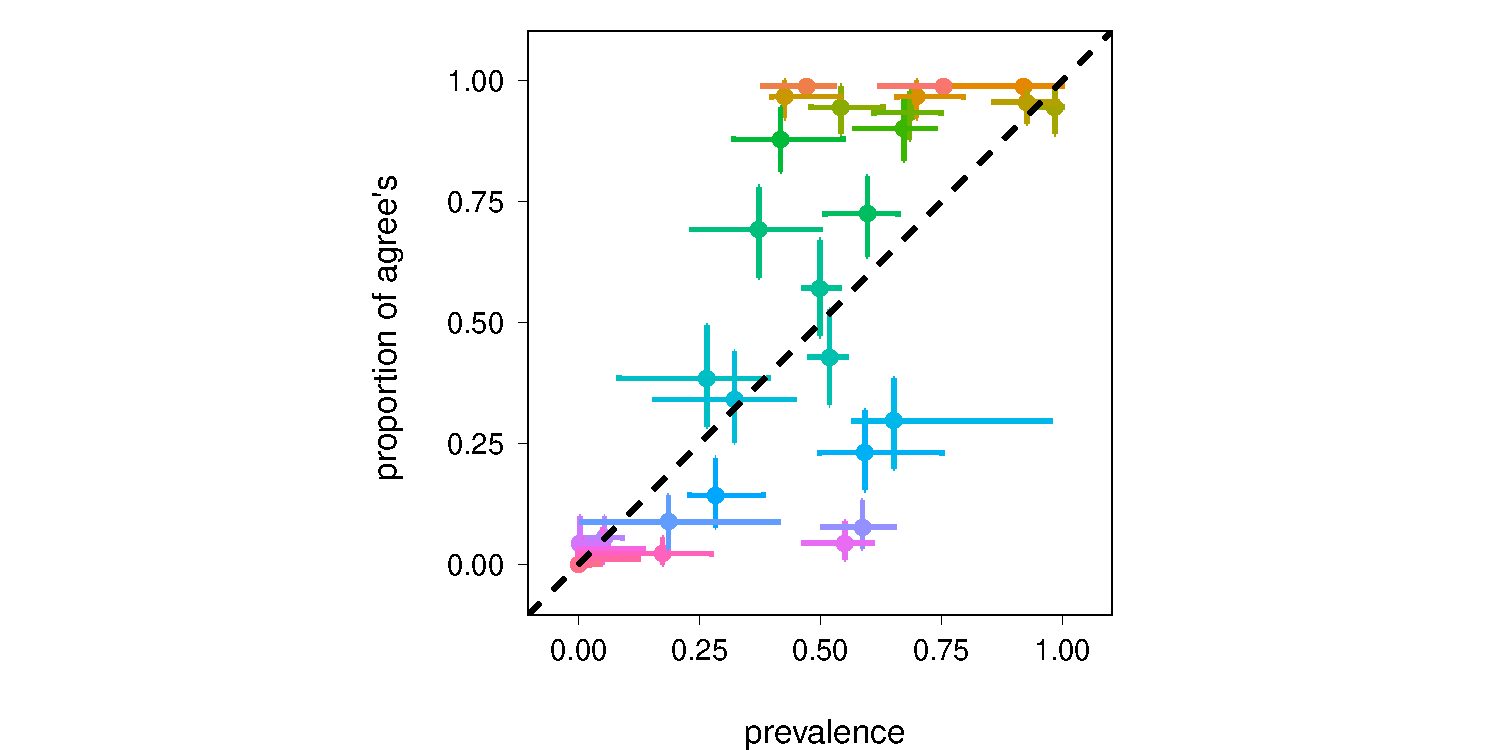
\includegraphics[width=\columnwidth]{tj_n100_tjVsprev_95hdi.pdf}
    \caption{Truth judgments from Expt.~1b for each item vs. the prevalence of the property for the target item as measured in Expt.~1a. For example, ``Leopards have spots'' has a very high truth judgment (Expt.~1b; Y-axis), and ``has spots'' is a highly prevalent property for leopards (Expt.~1a; X-axis). Color spectrum corresponds to the rank ordering of the truth judgment data; similarly colored dots received similar truth judgments.}
  \label{fig:scatterprev}
\end{figure}




\subsection{Lifted-variable model predictions}

The speaker model specified in Section \ref{sec:model} reasons about the likely prevalence that a listener will infer given  a generic sentence and assuming an informative speaker and a distribution over the prevalence of the property. 
In this way, the model takes into account the prevalence of the property both within- and across-categories as well as communicative principles.
We explore the predictions of this model, using the empirical priors elicited in Expt.~1a. 
We compare these predictions to the truth judgment data observed in Expt.~1b.
\subsubsection{Priors}

The model of generic language has 1 parameter: the speaker optimality parameter $\lambda$. We put an uninformative prior over this parameter, with a range consistent with previous literature using the same model class.

$$
\lambda \sim \text{Uniform}(0,1)
$$

In addition, we include a data-analytic ``contamination'' parameter to account for data that is more consistent with a model of random guessing. 
Modeling random guessing explicitly is important for recovering reliable estimates of the parameters of the model, which would otherwise be contaminated by this data \cite{LW2014}.
The data is modeled as a mixture of behavior derived from the generics model and random guessing behavior. 
We put an informative prior over the mixture parameter $\phi$.

$$
\phi \sim \text{Uniform}(0,1)
$$


\subsubsection{Posterior over model parameters}

The full model has one free parameter, the speaker rationality $\lambda$ in Equation \ref{eq:S1}, and one data analytic parameter, a contamination parameter $\phi$.
To learn about the \emph{a posteriori} credible values of our model parameters, we used the probabilistic programming language WebPPL \cite{dippl} to collect 3 chains of 100,000 iterations removing the first 50,000 iterations using the Metropolis-Hastings algorithm. 
The speaker rationality parameter represents the speaker's belief in how rational the hypothetical listener believes he is when choosing to say the generic (over saying nothing). 
The 95\% Highest Probability Density (HPD) Interval is [3.36, 4.98].

In the data analysis, we also include a contamination parameter $\phi$ to account for noise in the data.  
This represents the proportion of the data that can be better explained by random guessing than by our model of generic language.
In this way, $\phi$ provides a crude measure of goodness of fit. 
The 95\% HPD Interval is [0.026,0.049]. 
This suggests that there is not a substantial amount of noise in the data, possibly owing to the simplicity of the task. 


\subsubsection{Posterior predictive}

We evaluate the model by examining the posterior predictive distribution of responses. The posterior predictive distribution marginalizes over the inferred parameter values to produce predictions about what the data should look like given the lifted-threshold model and the observed data. This is akin to fitting the parameters and is an important step in model validation: It shows what data is actually predicted by the model. 
Figure \ref{fig:modeldataScatter} shows the Maximum A-Posteriori (MAP) values of the model predictions compared against the observed data. 
The model predicts graded endorsements for the generic statements used in Expt.~1b. 


\section{Experiment 2a: \emph{Measuring $P(x)$ for unfamiliar categories}}

In this experiment, we measured participants' beliefs about the distribution of the prevalence of certain properties within- and across- animal kinds. 
We expanded the stimulus set from \citeA{Cimpian2010} which consisted of novel animal categories (e.g. glippets) and various properties (e.g. have orange legs; have broken legs).


\subsection{Participants}

We recruited 40 participants over Amazon's crowd-sourcing platform Mechanical Turk (MTurk).  Participants were restricted to those with US IP addresses and with at least a 95\% MTurk work approval rating. All participants were native English speakers. The experiment took about 5-7 minutes and participants were compensated \$0.75.

\subsection{Procedure and materials}

In Expt.~1a, participants filled out a table with rows corresponding to different animal kinds and columns corresponding to different properties. 
Pilot testing suggested this was a pragmatically strange setup for this paradigm: answering ``What percentage of lorches have purple feathers?'', when participants knew nothing about lorches was difficult.
We took advantage of the latent structure in the task, described in Section \ref{sec:bda1}, and used a Bayesian statistical model to infer the underlying distribution. 
We then used these distributions in our language model to make predictions about the implications of generic sentences.

Participants were asked about the prevalence across categories by asking them the likelihood of there existing a K that has F, where K was a novel animal category and F was a property (e.g. ``how likely is it that there is a lorch that is female?''). 
Prevalence within categories was measured by asking participants about the percentage of Ks that have Fs, given that at least one does.
Participants responded using slider bars that ranged from ``unlikely'' to ``likely'', and ``0\%'' to ``100\%'', respectively.
Complete instructions shown to participants are in Appendix \ref{sec:prior2instruct}. 

Materials---novel animal names and familiar properties---built upon those from \citeA{Cimpian2010}. 
Classic work in generalization suggested to us that there may be differences in the implications of generic statements of different types of biological properties \cite{Nisbett1983}. 
We expanded the stimulus set to include four different types of properties: biological parts (e.g. ``feathers''), colored parts (e.g. ``purple feathers''), vague parts (e.g. ``smooth feathers''), and accidental parts (e.g. ``broken feathers''). 
Pilot testing revealed a lot of variability across items in the accidental properties relative to the other types of properties. 
To test the quantitative predictive power of the generic interpretation model, we used twice as many exemplars of accidental properties, with the aim to make a ``common accidental'' and a ``rare accidental'' class of properties. 
We used 8 exemplars of each of the three non-accidental properties (``parts'', ``colored parts'', ``vague parts'') and 16 exemplars of accidental properties.
Materials are in Appendix \ref{sec:materials2}.

\subsection{Bayesian data analysis}
\ref{sec:bda2}
In order to recover single belief distributions representing prevalence both within- and across- categories (analogous to those elicited in Expt.~1a and shown in Figure \ref{fig:priors1a}), we built a simple Bayesian statistical model of the task questions and their relation to the desired distribution. 

Participants' responses to each question (slider bar values) were assumed to be samples from Beta distributions with unknown means and concentrations. 
The responses to the questions ($d_{across}, d_{within}$) were used to estimate the parameters of the distributions of prevalence across- and within- categories, separately. 
\begin{align*}
d_{across} \sim \text{Beta}(\gamma_{across}, \delta_{across}) \\
d_{within} \sim \text{Beta}(\gamma_{within}, \delta_{within}) 
\end{align*}
The parameters $\gamma$ and $\delta$ correspond to the mean and variance (formally, the concentration), respectively, of prevalence for each of the across- and within- distributions.
%As in our other models, we assume some global proportion of noise in the experimental data $\phi$. 
We put identical, uninformative priors on these parameters:
\begin{align*}
%\phi & \sim \text{Uniform}(0,1) \\
\gamma & \sim \text{Uniform}(0,1) \\
\delta & \sim \text{Uniform}(0,20) 
\end{align*}
To construct single prevalence distributions reflecting both the within- and across- category prevalence (as we have for Expt.~1a), we assume that the distribution is a mixture of categories that have the property and categories that don't have the property\footnote{This is similar in spirit to Hurdle Models of count data used in clinical trials where the observed proportion of zeros is greater than one would expect from classical models of count data like the Poisson model.}. Whether or not a category has a property ($h$) is driven by the prevalence across categories ($\theta_{across}$).
%
\begin{align*}
\theta_{across} & \sim \text{Beta}(\gamma_{across}, \delta_{across}) \\ 
h & \sim \text{Bernoulli}(\theta_{across}) \\
x & \sim \begin{cases} 
		\text{Beta}(\gamma_{within}, \delta_{within}) &\mbox{if } h = 1 \\ 
				0 & \mbox{if } h=0. 
				\end{cases} 
\end{align*}
%
Marginal posterior distributions for $x$ were estimated using the Metropolis-Hastings algorithm in the probabilistic programming language WebPPL \cite{dippl}. Inference was completed by taking 50,000 samples using the Metropolis-Hastings algorithm.

\section{Experiment 2b: mismatches between \emph{truth conditions} and \emph{implications}}

\citeauthor{Cimpian2010} observed that generic statements of novel kinds with biological properties (e.g. ``Glippets have yellow fur'') show an asymmetry between the conditions by which the generic is true (``\emph{truth conditions}'') and the prevalence implied by the generic (``\emph{implied prevalence}''). 
Generic sentences were endorsed for a wide-range of prevalence levels (e.g. when ``30\% of glippets have yellow fur.''), resulting in intermediate average truth conditions. 
Upon hearing a generic, listeners inferred that the property was widespread (e.g. almost all glippets have yellow fur).
This mismatch between \emph{truth conditions} and \emph{implied prevalence} was significantly reduced for generics of properties plausibly construed as accidental (e.g. ``Glippets have wet fur.'').

In this experiment,  we replicate these findings and extend them to reveal even more variability in the mismatch between \emph{truth conditions} and \emph{implied prevalence} using the types of properties from Expt.~2a.
We also show how the prevalence-based model predicts the variability in the mismatch with strong quantitative accuracy.


\subsection{Participants}

We recruited 80 participants over Amazon's crowd-sourcing platform Mechanical Turk (MTurk).  
Participants were restricted to those with US IP addresses and with at least a 95\% MTurk work approval rating. 
All participants were native English speakers. 
The experiment took about 5 minutes and participants were compensated \$0.60.

\subsection{Procedure and materials}

In order to get participants motivated to reason about novel animals, they were told they were the resident zoologist of a team of scientists that recently discovered an island with many new animals; their task was to provide their expert opinion on questions about these animals\footnote{The experiment in full can be viewed at \url{http://stanford.edu/~mtessler/generics/experiments/asymmetry/asymmetry-2.html}}. 
We recruited 40 participants for the \emph{truth conditions} task and 40 participants for the \emph{implied prevalence task}. 

Following \citeauthor{Cimpian2010}'s paradigm, in the \emph{truth conditions} task, participants were given an evidence statement consisting of the percentage of a novel animal category that had a property (e.g.~``30\% of glippets have yellow fur''). 
Participants were asked if they agreed or disagreed with the associated generic statement (i.e.~``Glippets have yellow fur.'').
Prevalence varied between 10, 30, 50, 70, and 90\%.
The experiment consisted of 25 trials: 5 trials for each of 5 types of properties measured in Expt.~2a (part, color part, vague part, common accidental, rare accidental). 
Each prevalence level appeared once for each property type (5 prevalence levels x 5 property types). 

Participants in the \emph{implied prevalence} task were supplied with the generic (e.g. ``Glippets have yellow fur.'') and asked to judge prevalence: ``What percentage of glippets do you think have yellow fur?''. Participants saw 25 trials: 5 for each of 5 property types.
The original study by \citeauthor{Cimpian2010} found a difference in the implied prevalence between ``color parts'' (e.g. yellow fur) and accidental properties (e.g. wet fur).
The prevalence priors inferred from Expt.~2a suggest that generic interpretation should be even more variable than simply strong vs. weak.
For this reason, we included three types of biological properties: parts (e.g. fur), color--part pairs (e.g. yellow fur) and gradable adjective--part pairs (e.g. curly fur). 
We also coded the accidental properties from Expt.~2a as either ``common'' or ``rare'' using a by-item median split.

 
Most of the materials we used were from \citeauthor{Cimpian2010}. 
The materials used were 30 novel animal categories (e.g. lorches, morseths, blins) each paired with a unique property. 
Biological properties were made by pairing a color with a body-part (e.g. purple feathers, orange tails). 
Accidental properties used the same set of body-parts but modified it with an adjective describing an accidental or disease state (e.g. broken legs, wet fur). 
Each participant saw a random subset of 10 unique animal-property pairs for each type of property (biological and accidental). 
Table \ref{tab:sampleTrial} shows an example trial for each of the property types and tasks.


\begin{table}[h]
\begin{tabular}{| l |  l | l | l |}
\hline
           &             & Truth conditions                                                                                                    & Implied prevalence                                            \\
           \hline \hline
Biological &             &                                                                                                                     &                                                               \\
\hline
           & Information & xx\% of lorches have purple feathers.                                                                               & Lorches have purple feathers.                                 \\
\hline
           & Question    & \begin{tabular}[c]{@{}l@{}}Is the following sentence true or false?\\ \\ Lorches have purple feathers.\end{tabular} & \begin{tabular}[c]{@{}l@{}}What percentage of lorches \\do you think have purple feathers?\end{tabular} \\
           \hline \hline
Accidental &             &                                                                                                                     &                                                               \\
\hline
           & Information & xx\% of lorches have muddy feathers.                                                                                & Lorches have muddy feathers.                                  \\
\hline
           & Question    & \begin{tabular}[c]{@{}l@{}}Is the following sentence true or false?\\ \\ Lorches have muddy feathers.\end{tabular}  & \begin{tabular}[c]{@{}l@{}}What percentage of lorches \\ do you think have muddy feathers?\end{tabular} \\
\hline
\end{tabular}
\caption{Sample item from Experiment 2}
\label{tab:sampleTrial}

\end{table}



\subsection{Lifted-variable model predictions}

In Expt.~1, the acceptability of the generic was modeled as a speaker (Eq.~\ref{eq:S2}) reasoning about whether or not to produce the generic given some known prevalence. 
We use the same model to make predictions for the \emph{truth conditions} data.
The \emph{implied prevalence} task is slightly different: Here, the participant hears a generic and is asked to infer the likely prevalence of the property. 
This is the model of the listener in Eq.~\ref{eq:L1}. 
We use this model to predict the data from the implied prevalence task.

\subsubsection{Priors}


Each of these models has a parameter governing the optimality of the hypothetical speaker in Eq.~\ref{eq:S1}. 
Since the supports of the distributions produced by the two models are different ($S_2$ returns a distribution over ``agree'' and ``disagree'', whereas $L_1$ generates a distribution prevalence levels), there is no reason to believe the speaker optimality parameters would be the same for the two models. 
Hence, we put independent prior distributions over the two parameters: $\lambda_{\text{truth conditions}}, \lambda_{\text{implied prevalence}} \sim \text{Uniform}(0, 20)$.

As before, we model the observed data as being generated by a mixture of our generics model and a model of random guessing behavior. 
We use a guessing parameter for each task independently, since guessing behavior is fundamentally different between the two tasks (\emph{truth conditions}: 50\% chance of choosing a particular response; \emph{implied prevalence}: 1\% chance of choosing a particular response).
We put an uninformative prior over these mixture parameter $\phi_{task} \sim \text{Uniform}(0,1)$, and infer its credible values from the data.

\subsubsection{Posteriors over model parameters}

To learn about the \emph{a posteriori} credible values of our model parameters, we used the probabilistic programming language WebPPL \cite{dippl} to collect 100,000 samples using the Metropolis-Hastings algorithm. 
The estimated posterior distributions of the contamination parameters $\phi_{task}$ are shown in Figure \ref{fig:phi2}. 
This parameter represents the proportion of the data that is better explained by a model of random guessing than by the prevalence-based generics model. 
The 95\% Credible interval is [0.06, 0.15]. 

\begin{figure}
\centering
    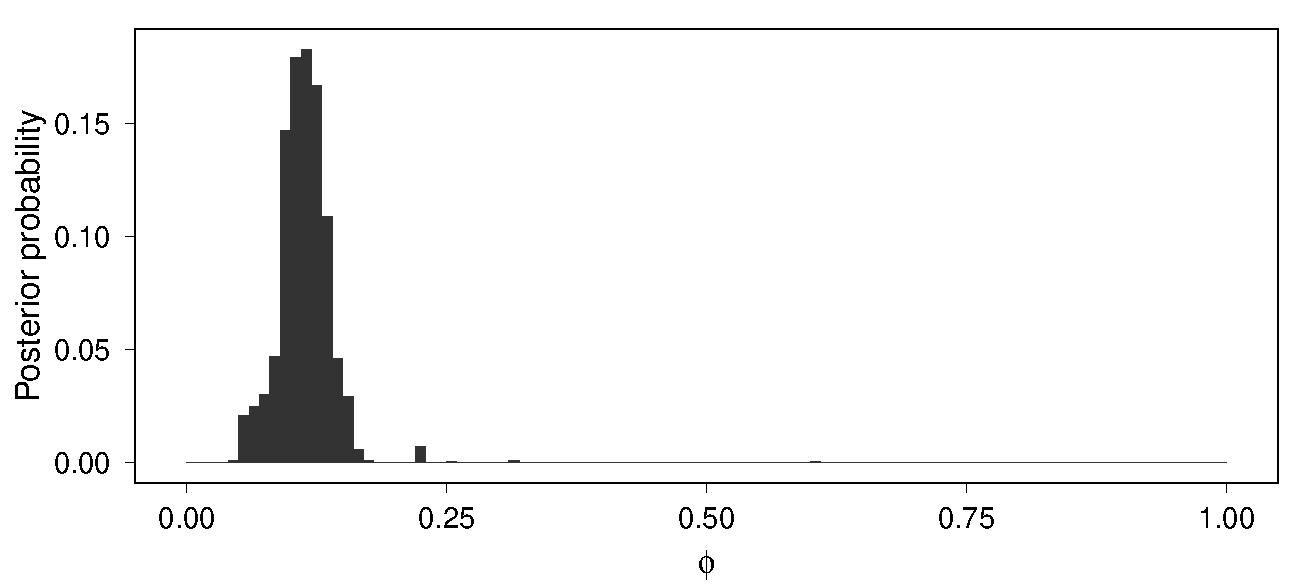
\includegraphics[width=0.8\columnwidth]{asym-phi-2opts-phi-100k.pdf}
    \caption{Posterior distribution of the contamination (``guessing'') parameter. The 95\% credible interval is [0.06, 0.15].}
  \label{fig:phi2}
\end{figure}

The estimated posterior distribution of the speaker rationality parameters $\lambda_{\text{truth conditions}}$ and $\lambda_{\text{implied prevalence}}$ are shown in Figure \ref{fig:rationality2}. 
This parameter represents the belief in how rational the hypothetical speaker in Eq.~{ref:eqS1} is believed to be when choosing to say the generic (over saying nothing). 
The 95\% credible interval for $\lambda_{\text{truth conditions}}$ is [0.23, 6.9] and $\lambda_{\text{implied prevalence}}$ is [1.30, 16.86]. The fact that these parameters are so different is expected given that the state space in the two tasks is also quite different.


\begin{figure}
\centering
    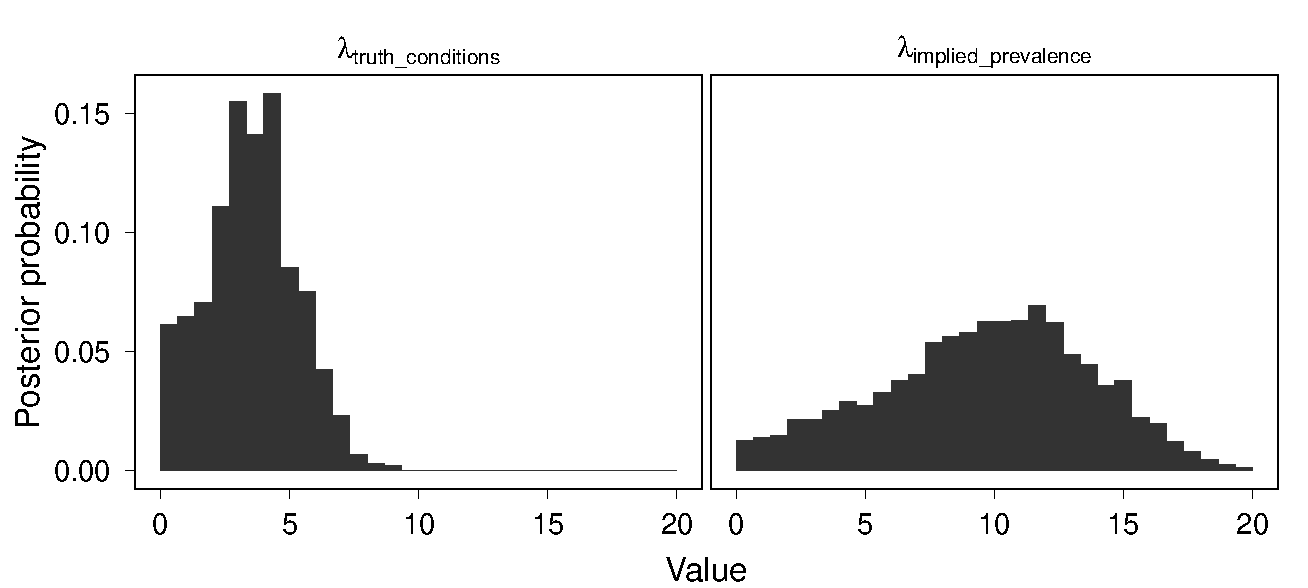
\includegraphics[width=0.8\columnwidth]{asym-lambdas-2opts-phi-100k.pdf}
    \caption{Posterior distribution of the speaker rationality parameters. The 95\% credible interval for $\lambda_{\text{truth conditions}}$ is [0.23, 6.9] and  $\lambda_{\text{implied prevalence}}$ is [1.30, 16.86]. The fact that these parameters are so different is expected given that the state space in the two tasks is also quite different.}
  \label{fig:rationality2}
\end{figure}






\section{Stimuli used in Experiment 1}
\label{sec:appendix}	

\begin{table}[h]
\begin{tabular}{| l | l | p{3.5cm} | p{3.5cm} |}
\hline
Conceptual type & Item & Truth judgment & Prevalence \\
\hline \hline
Majority characteristic       & 1. Leopards have spots.    &0.956	[0.912, 0.989] & 92.7 [85.9, 99.0]\\
                                          & 2. Ducks have wings.                       &0.945	[0.89, 0.989] & 98.5 [95.2, 99.9]\\
                                          & 3. Cardinals are red.                       &0.989	[0.967, 1] & 75.5 [62.1, 86.9]\\
                                          & 4. Swans are white.                       &0.901	[0.835, 0.967] & 67.3 [57.1, 73.8] \\
                                          & 5. Peacocks have beautiful feathers. &  0.989	[0.967, 1] & 92.0 [77.7, 100] \\
Minority characteristic       & 6. Lions have manes.       &0.945	[0.89, 0.989] & 54.3 [48.1, 63.0]\\
                                          & 7. Kangaroos have pouches.                        &0.967 [0.923, 1]& 69.9 [65.8, 79.6]\\
                                          & 8. Robins lay eggs.                        &0.934	[0.879, 0.978]& 68.5 [61.1, 74.9]\\
Striking                      & 9. Sharks attack swimmers. &0.879	[0.813. 0.945] & 41.8 [32.0, 54.7]\\
                                  & 10. Mosquitos carry malaria.                        &0.989	[0.967, 1] & 47.2 [38.1,	 52.9]\\
                                  & 11. Ticks carry Lyme disease.                        &0.967	[0.923, 1] &  42.6 [40.0, 54.2]\\
                                  & 12. Tigers eat people.                        &0.692	[0.593, 0.78] & 37.3 [23.3, 49.9]\\
False generalization & 13. Robins are female.      &0.429	[0.33, 0.527] & 51.9 [47.8. 55.4]\\
                                              & 14.  Lions are male.                       &0.571	[0.473, 0.67] & 49.9 [46.6, 53.9]\\
                                         & 15. Swans are full-grown. & 0.725	[0.637, 0.802] & 59.7[51.0, 66.0]\\
                                         & 16. Leopards are juvenile. & 0.143	[0.077,0.22] & 28.3 [22.9, 38.2] \\
                                         & 17. Sharks are white. & 0.341	[0.253, 0.44] & 32.2 [15.8, 44.6] \\
False or Uncertain & 18. Leopards have wings.       &0.022	[0, 0.055]& 1.0 [0.0, 4.1]\\
                                              & 19. Kangaroos have spots.                       & 0.033 [0, 0.077]& 5.0 [0.1, 13.5]\\
                                              & 20.  Tigers have pouches.                       &0.011	[0, 0.033]& 2.0 [0.0, 12.3]\\
                                              & 21.  Robins carry malaria.                       &0.055	[0.011, 0.099]& 5.4 [1.6, 9.1]\\
                                              & 22. Sharks have manes.                       &0.044	[0.011, 0.099]& 0.3 [0.0, 5.7]\\
                                              & 23. Lions lay eggs.                       &0 [0, 0] & 0.1 [0.0, 4.3]\\
                                              & 24. Sharks don't attack swimmers.                       &0.231 [0.154, 0.319] & 59.3 [49.8, 75.1]\\
                                              & 25. Ticks don't carry Lyme disease.                       &0.044 [0.011, 0.088] & 55.1 [46.6, 60.8]]\\
                                              & 26. Mosquitos don't carry malaria.                       &0.077 [0.033, 0.132] & 58.7 [50.5, 65.3]]\\                                              
                                              & 27. Tigers don't eat people.                       &0.297 [0.198, 0.385]& 65.3 [56.9, 97.7]\\                                              
                                              & 28. Peacocks don't have beautiful feathers.                       &0.022 [0, 0.055] & 17.4 [0.5, 27.5]\\                                              
                                               & 29. Mosquitos attack swimmers.       &0.385 [0.286, 0.495] & 26.5 [8.4, 39.2]\\
			                         & 30. Sharks lay eggs.       &0.088 [0.033, 0.143] & 18.5 [0.6, 41.3]\\
\hline

\end{tabular}
\caption{Stimuli used in Experiment 1. Estimates are means for truth judgments and Maximum A-Posteriori (MAP) estimates for prevalence.  Brackets denote 95\% confidence intervals for truth judgments and 95\% credible intervals for prevalences.}
\label{tab:expt1}
\end{table}


\section{Instructions used in Experiment 1a: prior elicitation for familiar categories}
\label{sec:prior1instruct}

Participants were told 
\begin{quote}
In this study, we are interested in how prevalent certain properties are within different kinds of animals. We will give you examples of the kinds of animals we have in mind and ask you to list a few of your own.

Then, you will estimate the \emph{percentage of the individual members} of the animal species that have certain properties.

On each trial, you will rate 8 properties. The properties will be revealed to you one at a time. Essentially, you will be filling out a big table. You are allowed to go back and revise your answers, if you think there is a more realistic estimate you could give. You will do this 2 times (2 big tables). 

\end{quote}


\section{Instructions used in Experiment 2a: prior elicitation for novel categories}
\label{sec:prior2instruct}

Participants were again told they were on a newly discovered island with lots of new animals on it. They were then given the following instructions

\begin{quote}
One day, you are roaming through the library when you encounter a data-collection robot. The robot doesn't know very much about the world and is asking you questions to learn more. Today, it wants to learn about properties of animals. It is randomly selecting an animal from its memory and a property from its memory, and asking you if the animal is likely to have the property.

Of course, you're new to this island so you don't really know anything about these animals. The properties, however, will be familiar. Try to provide your best guess given your own experience.
\end{quote}

Participants were then run through a practice trial where they were familiarized with the questions that would be asked on them. 
On each trial, the data-collection robot introduced a new animal (e.g. ``We recently discovered animals called glippets.''). 
The robot then asked how likely it was that ``there was \emph{a} glippet with [[property]]''. 
This question aimed to get at the prevalence of the property \emph{across} categories (e.g. it's very likely that there is a glippet that is female, less likely that there is a glippet that has wings, and even less likely that there is a glippet has purple wings). 
The second question was about the prevalence \emph{within} categories. The robot asked, ``Suppose there is a glippet that has wings. What percentage of glippets do you think have wings?''

\section{Stimuli used in Experiment 2}
\label{sec:materials2}

Many of these materials were originally used in \citeA{Cimpian2010}.

\begin{table}[h]
\begin{tabular}{| l || l | l | l |}
\hline
Property type               & Item                    & Across-category prevalence estimate  & Within-category prevalence estimate \\
\hline \hline
Body part       			& 1. Teeth    &  82.7	88.5	76.5 &                     \\
                                          & 2. Fur                       &78	80.5	68.9 &                     \\
                                          & 3. Tails                     &74.9	81.6	65&                     \\
                                          & 4. Claws                       &65.5	74.1	60.8&                     \\
                                          & 5. Feathers                       &67.6	74.3	61&                     \\
                                          & 6. Ears                       &85.4	89.1	80.2&                     \\
                                          & 7. Legs                       &88.3	92.8	81.2&                     \\
                                          & 8. Skin                       &89.5	93.1	85.1&                     \\
Colored part      	 & 9. Pink teeth       &                &                     \\
                                          & 10. Yellow fur                       &                &                     \\
                                          & 11. Orange tails                         &                &                     \\
                                          & 12. Blue claws                       &                &                     \\
                                          & 13. Purple feathers                      &                &                     \\
                                          & 14. Orange ears                    &                &                     \\
                                          & 15. Silver legs                       &                &                     \\
                                          & 16. Violet skin                      &                &                     \\       
Vague part      	 & 17. Long teeth       &                &                     \\
                                          & 18. Curly fur                       &                &                     \\
                                          & 19. Long tails                         &                &                     \\
                                          & 20. Big claws                       &                &                     \\
                                          & 21. Smooth feathers                      &                &                     \\
                                          & 22. Small ears                    &                &                     \\
                                          & 23. Long legs                       &                &                     \\
                                          & 24. Rough skin                      &                &                     \\ 
Common accidental part    & 25. Wet fur       &                &                     \\
                                          & 26. Dusty skin                       &                &                     \\
                                          & 27. Worn-out claws                         &                &                     \\
                                          & 28. Fungus-covered fur                      &                &                     \\
                                          & 29. Muddy feathers                      &                &                     \\
                                          & 30. Rotten teeth                   &                &                     \\
                                          & 31. Torn feathers                       &                &                     \\
                                          & 32. Itchy tails                      &                &                     \\  
Rare accidental part    & 33. Sore legs       &                &                     \\
                                          & 34. Torn tails                       &                &                     \\
                                          & 35. Cracked claws                         &                &                     \\
                                          & 36. Sore teeth                       &                &                     \\
                                          & 37. Swollen ears                      &                &                     \\
                                          & 38. Infected ears                    &                &                     \\
                                          & 39. Burned skin                       &                &                     \\
                                          & 40. Broken legs                     &                &                     \\                                                                                          
                                           \hline

\end{tabular}
\end{table}

\bibliographystyle{apacite}

\setlength{\bibleftmargin}{.125in}
\setlength{\bibindent}{-\bibleftmargin}

\bibliography{generics}

\end{document}

